\chapter{Appendix}

\section{Geographic Origin of All Cited Non-English Languages}\label{app:geo_origin}

In Figure~\ref{fig:geo_full} we show the geographic origin of cross-lingual citations in relative terms per cited language (i.e., the numbers of each \emph{row} add up to 1). The distinct diagonal of the matrix and the horizontal line for affiliations in English-speaking countries reflect the fact that most cross-lingual citations are either to a local language or originate from an English-speaking country. Among cited languages with a low number of total occurrences we can furthermore see a few cases showing unusual distributions, such as a single citation to Macedonian from an author affiliated with a Polish institution, or citations to Icelandic, where a single one originates from Iceland, while the remaining nine originate from institutions in countries where Japanese (3), Italian (1), and Swedish (5) are the most common language.

\begin{figure*}[tb]
\centering
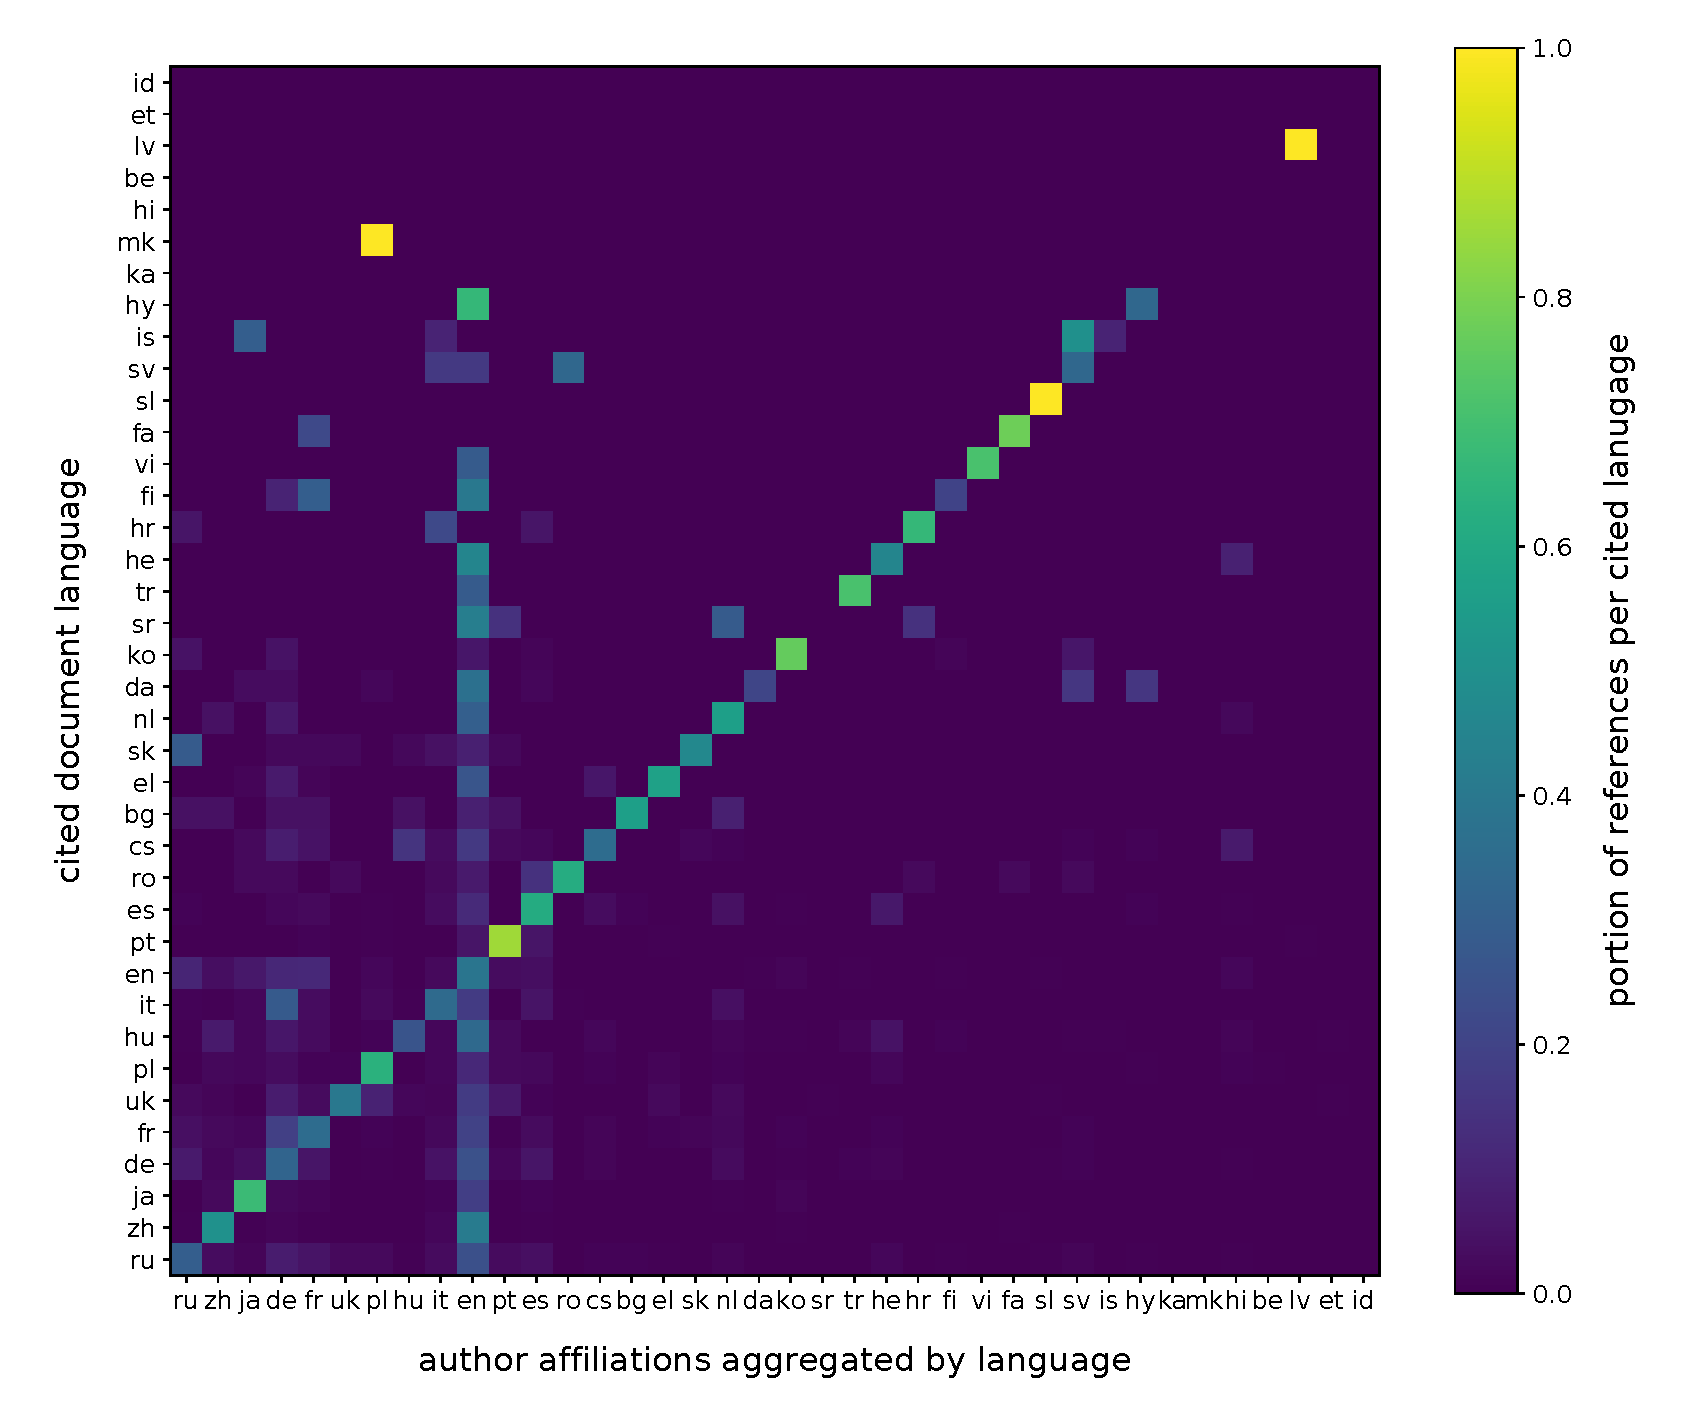
\includegraphics[width=\textwidth]{figures/ref_xling/citlang_to_author_aff_all_relative_crop.pdf}
\caption[Geographic origin of cross-lingual citations (relative count)]{Geographic origin of cross-lingual citations (relative count).} \label{fig:geo_full}
\end{figure*}

\section{Citation Intent and Sentiment Classification}\label{app:classifcation}

For the model training of both citation intent classification and citation sentiment classification, we fine-tune SciBERT uncased\refurl{https://huggingface.co/allenai/scibert_scivocab_uncased}{2024-01-10} using the following model configuration shown in Table~\ref{tab:modelconf}.

\begin{table}
\caption[Model configuration used for training]{Model configuration used for training.}
 \label{tab:modelconf}
  \centering
  \begin{small}
 \begin{threeparttable}
 \begin{tabular}{lr}
 \toprule
   Hyperparameter & value \\
   \midrule
  attention\_probs\_dropout\_prob &  0.1 \\
  gradient\_checkpointing &  false \\
  hidden\_act &  gelu \\
  hidden\_dropout\_prob &  0.1 \\
  hidden\_size &  768 \\
  initializer\_range &  0.02 \\
  intermediate\_size &  3072 \\
  layer\_norm\_eps &  1e-12 \\
  max\_position\_embeddings &  512 \\
  model\_type &  bert \\
  num\_attention\_heads &  12 \\
  num\_hidden\_layers &  12 \\
  pad\_token\_id &  0 \\
  position\_embedding\_type &  absolute \\
  transformers\_version &  4.4.2 \\
  type\_vocab\_size &  2 \\
  use\_cache &  true \\
  vocab\_size &  31090 \\
   \bottomrule
 \end{tabular}
\end{threeparttable}
  \end{small}
\end{table}

For determining the citation intent, we use the train, validation, and test split provided by the SciCite data set\refurl{https://huggingface.co/datasets/scicite}{2024-01-10} (train: 74\%, val: 8.3\%, test: 16.9\%). For citation sentiment, we split the Athar data set into train, validation, and test sets into 80\%, 10\%, and 10\%, respectively.



\section{HyperPIE Implementation Details}\label{app:hyperpie-implementation-details}

\paragraph{Fine-Tuned Models:}
We obtain the source code of PL-Marker from the author's GitHub repository\refurl{https://github.com/thunlp/PL-Marker/}{2024-01-10}. To make it work with our entity and relation schema, we extended the source code in \texttt{run\_acener.py} and \texttt{run\_re.py}. A patch file with all changes is provided in our code share. Our own RE model is a FFNN implemented with 4 hidden layers, each with ReLU activation and dimensions 300, 100, 25 and 2 respectively. All fine-tuned models are trained and evaluated on a local server with a GeForce RTX 3090 (24\,GB).

%  % MLPClassifier(
%  % hidden_layer_sizes=(300, 100, 25, 2),
%  % activation='relu',
%  % solver='adam',
%  % learning_rate_init=0.001,
%  % max_iter=90,
%  % random_state=1,
%  % shuffle=True,
%  % verbose=verbose

\paragraph{LLMs:}
GPT-3.5 was accessed through the official API. The total usage cost for all testing, prompt tuning, and the full evaluation runs sums up to 60\,USD. In zero-shot setting, all open models are run on a high performance compute cluster using the API layer Basaran.\refurl{https://github.com/hyperonym/basaran/}{2024-01-10} Vicuna and WizardLM  are run on nodes with $4\times$ NVIDIA Tesla V100 (32\,GB). GALACTICA and Falcon are run with half precision on nodes with $4\times$ NVIDIA A100 (80\,GB).

A zero-shot prompt example is shown in Listing~\ref{lst:promptexample}.

\begin{lstlisting}[language=plain,caption=Zero-shot prompt example.,label=lst:promptexample,breaklines=true,captionpos=b,frame=single,showlines=true,basicstyle=\tiny\ttfamily]
In the context of machine learning and related fields, what (if any) are the entities (datasets, models, methods, loss functions, regularization techniques) mentioned in the LaTeX Input Text below? What (if any) are their parameters and values?

[LaTeX Input Text start]
We use AdamW with a learning rate ($\alpha$) of 1e-3 for /* [...] */
[LaTeX Input Text end]

Answer in the following YAML format.

Format:
---
text_contains_entities: true/false
entities:
  - entity<N>:
      id: e<N>
      name: "<entity name>"
      type: dataset/model/method/loss function/regularization technique
      has_parameters: true/false
      parameters:
        - parameter<M>:
            id: p<N.M>
/* [...] */
...

Only include entities that are of type dataset, model, method, loss function, or regularization technique. Do not output entities that are of another type. Do not include entities of type task, metric, library, software, or API.
Only produce output in the YAML format specified above. Output no additional text.

Output:
\end{lstlisting}

For few-shot prompting, we employed 4\,bit quantization and used the \texttt{llama-cpp-python}\refurl{https://github.com/abetlen/llama-cpp-python/}{2024-01-10} API. % based on \texttt{llama.cpp}\footnote{See \url{https://github.com/ggerganov/llama.cpp/}.} backend with CUDA multi-GPU acceleration.
We use the default generation setup in \texttt{llama.cpp}
with parameters: temperature = 0, half precision = enabled, and repetition penalty = 1.1. A few-shot prompt example is shown in Listing~\ref{lst:fewshotprompt}.

\begin{lstlisting}[language=plain,caption=Few-shot prompt example.,label=lst:fewshotprompt,breaklines=true,captionpos=b,frame=single,showlines=true,basicstyle=\tiny\ttfamily]
### Instruction:
In the context of machine learning and related fields, what (if any) are the entities (datasets, models, methods, loss functions, regularization techniques) mentioned in the LaTeX Input Text below? What (if any) are their parameters and values?

Answer in the following YAML format.

Format:
```
has_entities: true/false
entities:
  - entity<N>:
      id: e<N>
      name: "<entity name>"
      type: dataset/model/method/loss function/regularization technique
      has_parameters: true/false
      parameters:
        - parameter<M>:
            id: p<N.M>
/* [...] */
```

Here are several examples.

### Example 1:

[LaTeX Input Text start]
We use AdamW with a learning rate ($\alpha$) of 1e-3 for /* [...] */
[LaTeX Input Text end]

### Response 1:
```
has_entities: true
  - entity1:
  	  id: e1
      name: "AdamW"
      has_parameters: true
      parameters:
        - parameter1:
            id: p1
/* [...] */
```

### Example 2:

[LaTeX Input Text start]
/* [...] */
[LaTeX Input Text end]

### Response 2:
```
/* [...] */
```

### Example 3:

[LaTeX Input Text start]
/* [...] */
[LaTeX Input Text end]

### Response 3:
```
/* [...] */
```

Only include entities that are of type dataset, model, method, loss function, or regularization technique. Do not output entities that are of another type. Do not include entities of type task, metric, library, software, or API.
Only produce output in the YAML format specified above. Output no additional text.

[LaTeX Input Text start]
We use AdamW with a learning rate ($\alpha$) of 1e-3 for /* [...] */
[LaTeX Input Text end]

### Response:
```
\end{lstlisting}

In the examples given in the few-shot prompts, we omitted the field \texttt{type: dataset/\allowbreak model/\allowbreak method/\allowbreak loss function/\allowbreak regularization technique}, because this information is not part of the gold annotation. As a consequence, the model outputs also tend to skip this attribute.

% \chapter{Bappendix}

% \section{Bar}
% \Blindtext
